\chapter*{Física}
\setcounter{chapter}{1}
\setcounter{section}{0}

\section{Vectores}
\setcounter{section}{0}

Para las magnitudes vectoriales (ejemplo: velocidad), no basta con saber su magnitud, sino que también es necesario saber su \textbf{dirección y sentido}. Para esto se utilizan los vectores.\\
Para medirlos se necesita un número real, llamado \textbf{cantidad} y un símbolo que define la unidad.\\

\begin{center}
    \begin{tabular}{|c|c|c|}
        \hline
        \multicolumn{3}{|c|}{\textbf{UNIDADES BÁSICAS DEL SISTEMA INTERNACIONAL}} \\
        \hline
        \textbf{Magnitud Física} & \textbf{Unidad} & \textbf{Símbolo} \\    
        \hline
        Longitud & metro & m \\
        \hline
        Masa & kilogramo & kg \\
        \hline
        Tiempo & segundo & s \\
        \hline
        Intensidad de corriente eléctrica & amperio & A \\
        \hline
        Temperatura & kelvin & K \\
        \hline
        Cantidad de materia & mol & mol \\
        \hline
        Intensidad luminosa & candela & cd \\
        \hline
        Ángulo plano & radian & rad \\
        \hline
        Ángulo sólido & estereorradian & sr \\
        \hline
    \end{tabular}
\end{center}

\begin{center}
    \begin{tabular}{|c|c|c|c|c|}
        \hline
        \multicolumn{5}{|c|}{\textbf{UNIDADES DERIVADAS DEL SISTEMA INTERNACIONAL}} \\
        \hline
        \textbf{Magnitud} & \textbf{Nombre} & \textbf{Símbolo} & \textbf{Derivadas} & \textbf{Básicas} \\
        \hline
        Frecuencia & Hertz & Hz &  & s$^{-1}$ \\
        \hline
        Fuerza & Newton & N &  & mkgs$^{-2}$ \\
        \hline
        Presión & Pascal & Pa & N/m^2 & mkgs$^{-2}$ \\
        \hline
        Energía & Joule & J & Nm & $m^2kgs^{-2}$ \\
        \hline
        Potencia & Watt & W & J/s & $m^2kgs^{-3}$ \\
        \hline
        Carga eléctrica & Coulomb & C &  & sA \\
        \hline
        Tensión eléctrica & Volt & V & W/A & $m^2kgs^{-3}A^{-1}$ \\
        \hline
        Resistencia eléctrica & Ohm & $\Omega$ & V/A & $m^2kgs^{-3}A^{-2}$ \\
        \hline
        Conductancia eléctrica & Siemens & S & A/V & $m^{-2}kgs^{3}A^{2}$ \\
        \hline
        Capacitancia & Farad & F & C/V & $m^{-2}kgs^{4}A^{2}$ \\
        \hline
        Flujo magnético & Weber & Wb & Vs & $m^2kgs^{-2}A^{-1}$ \\
        \hline
        Inductancia & Henry & H & Wb/A & $m^2kgs^{-2}A^{-2}$ \\
        \hline
        Inducción magnética & Tesla & T & Wb/m^2 & $kgs^{-2}A^{-1}$ \\
        Flujo luminoso & Lumen & lm &  & $cdsr$ \\
        \hline
        Intensidad luminosa & Lux & lx & lm/m^2 & $cdsr^{-2}$ \\
        \hline
        Temperatura Celcius & Grados Celsius & $^\circ$ C &  & K \\
        \hline
    \end{tabular}
\end{center}

Los prefijos para la formación de múltiplos y submúltiplos de las unidades básicas son los siguientes:
\begin{center}
    \begin{tabular}{c|c|c}
        Factor & Prefijo & Símbolo \\
        \hline
        $10^{18}$ & exa & E \\
        $10^{15}$ & peta & P \\
        $10^{12}$ & tera & T \\
        $10^{9}$ & giga & G \\
        $10^{6}$ & mega & M \\
        $10^{-6}$ & micro & $\mu$ \\
        \hline
        $10^{3}$ & kilo & k \\
        $10^{2}$ & hecto & h \\
        $10^{1}$ & deca & da \\
        $10^{-1}$ & deci & d \\
        $10^{-2}$ & centi & c \\
        $10^{-3}$ & mili & m \\
        \hline
    \end{tabular}
\end{center}

Unidades de longitud, fuerza, capacidad, área y volumen:
\begin{center}
    \begin{tabular}{|c|c|c|c|c|c|c|}
        \hline
        \multicolumn{7}{|c|}{\textbf{Unidades de longitud}}\\
        \hline
        kM & hM & daM & m & dM & cM & mM \\
        \hline
    \end{tabular}
    \vspace{0.5cm}
    \begin{tabular}{|c|c|c|c|c|}
        \hline
        \multicolumn{5}{|c|}{\textbf{Unidades de fuerza}}\\
        \hline
        kN & daN & N & dN & mN \\
        \hline
    \end{tabular}
    \vspace{0.5cm}
    \begin{tabular}{|c|c|c|c|c|c|c|}
        \hline
        \multicolumn{7}{|c|}{\textbf{Unidades de capacidad}}\\
        \hline
        kL & hL & daL & L & dL & cL & mL \\
        \hline
    \end{tabular}
    \vspace{0.5cm}
    \begin{tabular}{|c|c|c|c|c|c|c|}
        \hline
        \multicolumn{7}{|c|}{\textbf{Unidades de área}}\\
        \hline
        $km^2$ & $hm^2$ & $dam^2$ & $m^2$ & $dm^2$ & $cm^2$ & $mm^2$ \\
        \hline
    \end{tabular}
    \vspace{0.5cm}
    \begin{tabular}{|c|c|c|c|c|c|c|}
        \hline
        \multicolumn{7}{|c|}{\textbf{Unidades de volumen}}\\
        \hline
        $km^3$ & $hm^3$ & $dam^3$ & $m^3$ & $dm^3$ & $cm^3$ & $mm^3$ \\
        \hline
    \end{tabular}
\end{center}

\section{Vectores geométricos}
\blueBox{Definición}{
    Se le dice \textbf{vector} a todo segmento orientado. El primer punto es el \emph{origen} y el otro es el \textbf{extremo}.
}

\begin{center}
    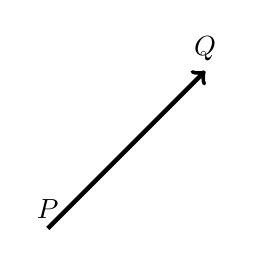
\begin{tikzpicture}
        \draw[->, ultra thick] (0,0) -- (2,2);
        \node[above] at (0,0) {$P$};
        \node[above] at (2,2) {$Q$};
    \end{tikzpicture}
    % text PQ with an arrow above it
    Figura: Vector $\vect{PQ}$ 
\end{center}

Dos vectores son \textbf{paralelos} cuando tienen la misma dirección. La dirección está dada por la recta que contiene al vector. El sentido está dado por el origen y el extremo.

\blueBox{Módulo de un vector}{
    Se llama \textbf{módulo} de un vector a la longitud del segmento orientado que lo define. al módulo de un vector $\vect{v}$ se lo denota como:
    $$|| \vect{v} ||$$
}

\blueBox{Vectores equivalentes}{
    Dos vectores son \textbf{equivalentes} cuando tienen el mismo módulo, dirección y sentido.
}

Para la suma de vectores se puede aplicar la \textbf{"regla del paralelogramo"}: dados dos vectores $\vect{v}$ y $\vect{w}$ con origen en el mismo punto, se hace un paralelogramo trazando por el extremo de $\vect{w}$ una paralela a $\vect{v}$ y también del otro lado. La suma ("resultante") es el vector que tiene su origen en el mismo punto que los otros dos y su extremo en el punto de intersección de las dos paralelas.

\begin{center}
    \includegraphics[width=0.5\linewidth]{regla_paralelogramo.jpg}
\end{center}
Simplificando: 
\begin{center}    
    \includegraphics[width=0.5\linewidth]{regla_paralelogramo2.jpg}
\end{center}

Para sumar más vectores, hay que poner al siguiente de manera que el origen sea el extremo del anterior.\\
Según la regla anterior puede ocurrir que al sumar vectores el origen del primero de
ellos coincida con el extremo del último:
\begin{center}    
    \includegraphics[width=0.7\linewidth]{regla_paralelogramo3.jpg}
\end{center}
\begin{center}    
    \includegraphics[width=0.5\linewidth]{regla_paralelogramo4.jpg}
\end{center}

\blueBox{Vector nulo y opuesto de un vector}{
    Un \textbf{vector nulo} es todo aquel que tiene módulo 0. Geométricamente es un punto y por eso no tiene ni sentido ni dirección.\\
    El \textbf{vector opuesto} de un vector $\vect{v}$ es el vector $-\vect{v}$ que tiene el mismo módulo y dirección que $\vect{v}$ pero sentido contrario.
}

\textbf{Propiedades de la suma de vectores}:
\begin{enumerate}
    \item Es asociativa: 
    $$\left( \vect{v_1} + \vect{v_2} \right) + \vect{v_3} = \vect{v_1} + \left(\vect{v_2} + \vect{v_3}\right)$$
    \item Es conmutativa: $\vect{v} + \vect{w} = \vect{w} + \vect{v}$
    \item El vector nulo respecto a la suma: $\vect{v} + \vect{0} = \vect{v}$
    \item $\vect{v} + (- \vect{v}) = \vect{0}$
\end{enumerate}

\blueBox{Resta de vectores}{
    Se llama \textbf{diferencia} $\vect{v} - \vect{w}$ de dos vectores, a la suma de un vector $\vect{v}$ y el opuesto de $\vect{w}$. Es decir,
    $$\vect{v} - \vect{w} = \vect{v} + (- \vect{w})$$
}
\begin{center}
    \includegraphics[width=0.6\linewidth]{diferencia_vectores.jpg}
\end{center}

\blueBox{Producto de un vector por un escalar}{
    El \textbf{producto} de un vector $\vect{v}$ por un escalar $k$ es el vector $k \vect{v}$ que tiene el mismo sentido y dirección que $\vect{v}$ pero módulo $|k|$ veces mayor. Si $k > 0$, el sentido es el mismo de $\vect{v}$, pero si $k < 0$, el sentido es el contrario al de $\vect{v}$\\
    Además, si $k = 0$ o $\vect{v} = \vect{0}$, entonces $k \vect{v} = \vect{0}$
}

\section{Vectores en el plano}

\begin{center}
    \begin{tikzpicture}
        \begin{axis}[
            axis lines = middle,
            ymin= -0.5, ymax=5,
            xmin= -0.5, xmax=6,
            xtick={4}, ytick={2}
        ]
            \draw[dashed] (4,0) -- (4,2) -- (0,2);
            \draw[->, ultra thick] (0,0) -- (4,2) node[midway, above] {$\vect{v}$};
            \draw[->, ultra thick] (2,2.5) node[below] {$P$} -- (5,4) node[above] {$Q$} ;
        \end{axis}
    \end{tikzpicture}
\end{center}

Las coordenadas de $\vect{PQ}$ son las coordenadas del extremo de $\vect{v}$, es decir (4,2). Se escribe: $\vect{PQ} = (4,2)$\\
Viendo los vectores en el sistema de coordenadas, es mucho más fácil. \\
Considerando los vectores $\vect{v} = (x_1, y_1)$ y $\vect{w} = (x_2, y_2)$, la suma está dada por:
$$\vect{v} + \vect{w} = (x_1 + x_2, y_1 + y_2)$$

\begin{center}
    \includegraphics[width=0.5\linewidth]{suma_vect_grafico.jpg}
\end{center}

Si $k \in \R$, entonces
$$k \vect{v} = (k \cdot x_1, k \cdot y_1)$$

Si $P$ y $Q$ son dos puntos en el plano, para obtener los componentes del vector $\vect{PQ}$, solo hay que hacer:
$$\vect{OP} + \vect{PQ} = \vect{OQ}$$
$$\vect{PQ} = \vect{OQ} - \vect{OP}$$

\begin{center}
    \includegraphics[width=0.5\linewidth]{componentes_vect_grafico.jpg}
\end{center}

\section{Módulo de un vector}

\begin{center}
    \begin{tikzpicture}
        \begin{axis}[
            axis lines = middle,
            ymin= -0.5, ymax=3,
            xmin= -0.5, xmax=6,
            xtick={4}, ytick={2},
            xticklabels={$x_1$}, yticklabels={$y_1$},
            xlabel={x}, ylabel={y}
        ]
            \draw[dashed] (4,0) -- (4,2) -- (0,2);
            \draw[->, ultra thick] (0,0) -- (4,2) node[midway, above, rotate=45] {$\sqrt{x^2_1 + y^2_1}$};
        \end{axis}
    \end{tikzpicture}
\end{center}

Si $\vect{v} = (x_1, y_1)$, entonces, según el Teorema de Pitágoras, $||\vect{v}|| = \sqrt{x^2_1 + y^2_1}$\\

\textbf{Propiedad de la longitud de un vector}:
\begin{enumerate}
    \item $||k \vect{v}||$ = $|k| \cdot ||\vect{v}||$
    \item (Desigualdad triangular) $||\vect{v} + \vect{w}|| \leq ||\vect{v}|| + ||\vect{w}||$
\end{enumerate}

\blueBox{Vector unitario}{
    Un vector es \textbf{unitario} o un \textbf{versor} si tiene módulo 1.\\
    \textbf{Normalizar} un vector no nulo es encontrar otro vector unitario que tenga la misma dirección y sentido que el vector dado.
}
Para normalizar un vector $\vect{v}$ debemos encontrar otro vector $\vect{w}$ tal que $\vect{w} = k \vect{v}$ con $k \in \R$ y $||\vect{w}|| = 1$. Teniendo en cuenta que:
$$1 = ||\vect{w}|| = || k \cdot \vect{v} || = |k| \cdot || \vect{v} ||$$
resulta que el $k$ necesario tiene que ser:
$$|k| = \frac{1}{||\vect{v}||}$$
Para que conserve el sentido, vamos a ir con:
$$k = \frac{1}{||\vect{v}||}$$

\textbf{Ejemplo:} queremos normalizr el vector $\vect{v} = (1,3)$. Primero calculamos el módulo:
$$||\vect{v}|| = \sqrt{1^2 + 3^2} = \sqrt{10}$$
Ahora, calculamos el $\vect{w}$:
$$\vect{w} = \left(\frac{1}{\sqrt{10}}, \frac{3}{\sqrt{10}}\right)$$

\blueBox{Vectores $\vect{i}, \vect{j}$}{
    $$\vect{i} = (1,0)$$
    $$\vect{j} = (0,1)$$
    \tcblower
    \textbf{Ejemplo:} Si $\vect{v} = 3\vect{i} + 4\vect{j}$, entonces $\vect{v} = 3(1,0) + 4(0,1) = (3,4)$
}

\section{Producto escalar}
Nueva operación: \textbf{$\R^2$}, el producto escalar. Nos va a dar como resultado un escalar, el ángulo.

\blueBox{Definición - Producto escalar}{
    Dados dos vectores $\vect{v}$ y $\vect{w}$, el \emph{producto escalar} entre estos vectores es:
    $$\vect{v} \cdot \vect{w} = \begin{cases}
        0 & \text{si $\vect{v}$ = 0 o  $\vect{w}$ = 0}\\
        ||\vect{v}|| \cdot ||\vect{w} || \cdot \cos \alpha & \text{si $\vect{v}$ y $\vect{w}$ no son nulos}
    \end{cases}$$
    Donde $\alpha$ es el ángulo entre $\vect{v}$ y $\vect{w}$.
}

\begin{center}
    \includegraphics[width=0.5\linewidth]{producto_escalar.jpg}
\end{center}
Considerando el triángulo anterior ($P, Q$ y $O$), tenemos que, mediante el teorema del coseno:
$$||\vect{PQ}||^2 = ||\vect{v}||^2 + ||\vect{w}||^2 - 2 \cdot ||\vect{v}||\cdot ||\vect{w}||\cdot \cos \alpha$$
Como $\vect{PQ} + \vect{v} = \vect{w}, \vect{PQ} = \vect{w} - \vect{v}$ y teniendo en cuenta que $\vect{v} = (v_1,v_2)$ y $\vect{w} = (w_1,w_2)$, tenemos que:
\begin{align*}
    2 \cdot ||\vect{v}|| \cdot ||\vect{w}|| \cdot \cos \alpha &= ||\vect{v}||^2 + ||\vect{w}||^2 - ||\vect{PQ}||^2\\
    &= v^2_1 + v^2_2 + w^2_1 + w^2_2 - ((w_1 - v_1) ^2 + (w_2 - v_2)^2)\\
    &= 2v_1w_1 + 2v_2w_2
\end{align*}
$$\boxed{\vect{v} \cdot \vect{w} = v_1w_1 + v_2w_2}$$
\textbf{Ejemplo:} Determinar el ángulo entre los vectores $\vect{v} = (-1,4)$ y $\vect{w} = (3,2)$
$$(-1,4)(3,2) = ||(-1,4)|| \cdot ||(3,2)|| \cdot \cos \alpha \Leftrightarrow -3 +8 = \sqrt{17} \sqrt{13} \cos \alpha$$
$$\frac{5}{\sqrt{221}} = \cos \alpha \Leftrightarrow \boxed{\alpha = 70,35^\circ}$$

\blueBox{Teorema}{
    Dos vectores no nulos son \textbf{perpendiculares} si y solo si su producto escalar es igual a 0
}
\blueBox{Vectores ortogonales}{
    Dos vectores son \textbf{ortogonales} si su producto escalar es cero.\\
    El vector nulo es ortogonal a todos los demás vectores.
}

\textbf{Propiedades del producto escalar}:
\begin{enumerate}
    \item $\vect{v} \cdot \vect{w} = \vect{w} \cdot \vect{v}$
    \item $\vect{u} \cdot (\vect{v} + \vect{w}) = \vect{u} \cdot \vect{v} = \vect{u} \cdot \vect{w}$
    \item $k(\vect{v} \cdot \vect{w}) = (k\vect{v}) \cdot \vect{w} = \vect{v} \cdot (k\vect{w})$
    \item $\vect{v} \cdot \vect{v} > 0$ si $\vect{v} \neq \vect{0}$ y $\vect{v} \cdot \vect{v} = 0$ si $\vect{v} = \vect{0}$
\end{enumerate}

\section{Proyección ortogonal}
Teniendo dos vectores, $\vect{v}$ y $\vect{w}$, hay que determinar $\vect{w_1}$ y $\vect{w_2}$, tal que:
\begin{enumerate}
    \item $\vect{v} = \vect{w_1} + \vect{w_2}$
    \item $\vect{w_1} || \vect{w}$
    \item $\vect{w_1} \perp \vect{w_2}$
\end{enumerate}

\begin{center}
    \includegraphics[width=0.5\linewidth]{proy_ortogonal.jpg}
\end{center}
El vector $\vect{w_2}$ es la \emph{componente vectorial de } $\vect{v}$ \emph{ortogonal a } $\vect{w}$.\\

Como los vectores $\vect{w_1}$ y $\vect{w}$ son paralelos, existe un escalar $k \in \R$ tal que $\vect{w_1} = k \cdot \vect{w}$. Por lo tanto, para determinar la proyección de $\vect{v}$ sobre $\vect{w}$, tenemos que calcular $k$. Empezaremos por la definición $\vect{v}$:
$$\vect{v} = \vect{w_1} + \vect{w_2}$$
$$\vect{v} = k \cdot \vect{w} + \vect{w_2}$$
Multiplicando ambos miembros por $\vect{w}$ y teniendo en cuenta que $\vect{w} \perp \vect{w_2}$ (multiplicarlos es igual a 0):

\begin{align*}
    \vect{v} \cdot \vect{w} &= (k \cdot \vect{w} + \vect{w_2}) \cdot \vect{w}\\
    \vect{v} \cdot \vect{w} &= (k \cdot \vect{w}) \cdot \vect{w} + (\vect{w_2} \cdot \vect{w})\\
    \vect{v} \cdot \vect{w} &= k \cdot (\vect{w} \cdot \vect{w}) + 0\\
    \vect{v} \cdot \vect{w} &= k \cdot ||\vect{w}||^2
\end{align*}
Por ende: 
$$k = \frac{\vect{v} \cdot \vect{w}}{||\vect{w}||}^2$$
y, finalmente
$$\boxed{\vect{w_1} = \text{proy}_{\vect{w}}\vect{v} = \frac{\vect{v} \cdot \vect{w}}{||\vect{w}||^2} \cdot \vect{w}}$$
Vamos a sacar el módulo del vector proyección:
$$||\text{proy}_{\vect{w}}\vect{v}|| = \left\| \frac{\vect{v} \cdot \vect{w}}{||\vect{w}||^2} \cdot \vect{w} \right\| = \frac{|\vect{v} \cdot \vect{w}|}{||\vect{w||^2}} \cdot ||\vect{w}|| = \frac{|\vect{v} \cdot \vect{w}|}{||\vect{w}||}$$
$$||\text{proy}_{\vect{w}} \vect{v}|| = ||\vect{v}|| \cdot |\cos \alpha|$$

\section{Aplicaciones matemáticas a la estática}

\textbf{Nociones elementales de estática}
\blueBox{Concepto de fuerza}{
    La \textbf{fuerza} es la acción ejercida sobre un cuerpo que cambia su forma y/o estado cinemático. Su efecto depende de la instensidad, dirección, sentido y punto de aplicación.\\
    La unidad que se usa para medir la intensidad (módulo) de una fuerza es \emph{Newton} ($N$).
    \tcblower
    Al conjunto de dos o más fuerzas sobre un cuerpo se le llama \textbf{sistema de fuerzas}.
}
\begin{center}
    \includegraphics[width=0.5\linewidth]{fuerza.jpg}
\end{center}
\begin{itemize}
    \item $|\vect{F}|$: Intensidad
    \item $r$: Recta de acción (dirección)
    \item Flecha: Sentido
    \item $P$: Punto de aplicación
\end{itemize}

\blueBox{Definición}{
    Un \emph{punto material o partícula} es el cuerpo que se está tratando como si fuese un punto geométrico, sin dimensión.
}
Un sistema de fuerzas plano o espacial se llama \emph{concurrente} si las rectas de acción de todas las fuerzas pasan por el mismo punto. De lo contrario, es \emph{no concurrente}.
\begin{center}
    \includegraphics[width=0.7\linewidth]{sist_fuerzas.jpg}
\end{center}

\textbf{Sistemas planos de fuerzas concurrentes}
Si el sistema está constituido por dos fuerzas y sus rectas de acción pasan por el mismo punto, puede ser reducido a un sistema de una fuerza, cuya recta pasa por el mismo punto que compartían las otras dos fuerzas y se determina por la regla del paralelogramo.
\begin{center}
    \includegraphics[width=0.9\linewidth]{fuerzas_concurrentes.jpg}
\end{center}
Para \textbf{equilibrar} este sistema, hay que agregarle una fuerza de igual intensidad (igual módulo), igual recta de acción y sentido opuesto a la fuerza $\vect{R}$. La vamos a llamar \emph{equilibrante} $\vect{E}$
\begin{center}
    \includegraphics[width=0.9\linewidth]{fuerzas_concurrentes2.jpg}
\end{center}

\textbf{Descomposición de una fuerza según dos direcciones concurrentes con ella.}\\
Se puede descomponer una fuerza con la regla del paralelogramo, siempre y cuando las 3 direcciones concurran a un mismo punto.\\
Si las direcciones son perpendiculares, se puede asociar un sistema de referencias ortogonal en donde la fuerza $\vect{F}$ se descomponga en las proyecciones de la misma sobre cada uno de los ejes coordenados.
\begin{center}
    \includegraphics[width=0.9\linewidth]{descomposicion_fuerzas.jpg}
\end{center}

\blueBox{Resolución analítica de sistemas planos de fuerzas}{
    Con un sistema caresiano de ejes $XY$, el vector de una fuerza puede ser indicado por su intensidad y el ángulo $\alpha$ que forma con el eje $X$. Su notación será $\vect{F} = (F, \alpha)$.\\
    La expresión cartesiana de la fuerza $\vect{F}$ resulta de analizar la proyección de la misma sobre cada uno de los ejes. La expresión analítica de una fuerza $\vect{F} = (F, \alpha)$ en un sistema cartesiano será:
    $$\vect{F}(x,y) = (F,\alpha) = F_x\vect{i} + F_y\vect{j} = (F \cos \alpha)\vect{i} + (F \sin \alpha)\vect{j} = (F_x, F_y)$$
    $\bf{F = ||\vect{F}||}$
}
\textbf{Ejemplo:} Dado el sitema de ejes cartesianos xy y las fuerzas: $\vect{F_1}(0,0) = (10N, 210^\circ)$ y $\vect{F_2}(0,0) = (20N, 60^\circ)$ determinen su expresión cartesiana.\\
Resolución:\\
Consideramos el módulo y ángulo de $\vect{F_1}$ para determinar sus proyecciones sobre los ejes:
$$\vect{F_1} = F_{1x}\vect{i} + F_{1y}\vect{j} = (10 \cos 210^\circ)\vect{i} + (10 \cos 210^\circ)\vect{j} = -5\sqrt{3}N\vect{i} - 5N\vect{j} = (-5\sqrt{3},-5)N$$
Por otro lado, hacemos lo mismo con las proyecciones de $\vect{F_2}$:
$$\vect{F_2} = F_{2x}\vect{i} + F_{2y}\vect{j} = (20 \cos 60^\circ)\vect{i} + (20 \sin 60^\circ)\vect{j} = 10N\vect{i} + 10\sqrt{3}N\vect{j} = (10,10\sqrt{3})N$$

\begin{center}
    \includegraphics[width=0.9\linewidth]{descomposicion_ejemplo.jpg}
\end{center}

\blueBox{Ecuaciones generales de equilibrio}{
    Para que un sistema plano de fuerzas concurrentes esté en equilibrio es necesario y suficiente que se verifiquen las siguientes igualdades:
    \begin{align*}
        \sum^n_{i=1} F_{ix}  = \sum^n_{i=1}F_i \cos \alpha_i = 0 & \:\:\: (\text{ecuación de proyección sobre } x)\\
        \sum^n_{i=1} F_{iy}  = \sum^n_{i=1}F_i \sin \alpha_i = 0 & \:\:\: (\text{ecuación de proyección sobre } y)\\
    \end{align*}
}

\textbf{Ejemplo:} Dado el sistema plano de fuerzas concurrentes, comprobar analíticamente el equilibrio.
$$\vect{F_1} = (5N, 270^\circ) \;\; \vect{F_2} = (\sqrt{52}N, 146,3^\circ) \;\; \vect{F_3} = (7N, 0^\circ) \;\; \vect{F_4} = (\sqrt{2}N, 135^\circ)$$
Resolución:\\
Se plantean las dos ecuaciones de proyección, sobre los ejes $x$ e $y$:
$$\sum^4_{i=1}F_{ix} = \sum^4_{i=1}F_{i} \cos \alpha_i = 5N \cos 270^\circ + \sqrt{52}N \cos 146,3^\circ + 7N \cos 0^\circ + \sqrt{2}N \cos 135^\circ$$
$= 0N-6N+7N-1N = 0N$
$$\sum^4_{i=1}F_{iy} = \sum^4_{i=1}F_{i} \sin \alpha_i = 5N \sin 270^\circ + \sqrt{52}N \sin 146,3^\circ + 7N \sin 0^\circ + \sqrt{2}N \sin 135^\circ$$
$= 5N+4N+0N+1N = 0N$

Ambas ecuaciones son iguales a cero, por lo que el sistema está en equilibrio.

\section{Cinemática del punto material}
Los problemas que resuelve la cinemática son, fundamentalmente, determinar la posición, desplazamiento, velocidad y aceleración de un objeto en función del tiempo.

\subsection{Movimiento}
La \textbf{posición} es la localización de un cuerpo en el espacio con respecto al sistema de referencia.\\
El \textbf{movimiento} es un cambio constante de posición en base a un sistema de referencia fijo.\\
Si el sistema no está fijo, se mide el movimiento relativo de un cuerpo con respecto a otro.\\
En todo movimiento hay que distinguir tres elementos fundamentales: el cuerpo que se
mueve o \underline{móvil}, el \underline{sistema de referencia} que se emplea y la \underline{trayectoria}.

\subsection{El móvil: una partícula o punto material}
La posición de un punto respecto de un sistema de referencia viene determinada por un \textbf{vector}. El estudio del movimiento del punto se reduce al estudio geométrico de dicho punto.\\
Un cuerpo cuyas dimensiones son despreciables frente al vector de posición es una
\textbf{partícula}

\subsection{Sistema de referencia. Vector posición}
Para conocer la posición de un punto en cualquier momento es necesario fijar otro punto como referencia.\\
Normalmente el punto de referencia será el 0, de los ejes cartesianos. (siempre teniendo en cuenta que el movimiento es en 2 dimensiones)\\
La posición del punto $P$ en cualquier instante vendrá determinada por el vector que une el punto de referencia con el punto móvil. El vector se llama \textbf{vector posición} y se denota por $\vect{r}$.

\begin{center}
    \begin{tikzpicture}
        \begin{axis}[
            axis lines=middle,
            xmin=0, xmax=6,
            ymin=0, ymax=6,
            xtick={1,4},
            ytick={1,2},
            xlabel=$x$,
            ylabel=$y$,
            xticklabels={$i$, x},
            yticklabels={$j$, y},
        ]
            \draw[dashed] (4,0) -- (4,2) -- (0,2);
            \draw[->, line width=0.7mm] (0,0) -- (4,2) node[above, right] {$P(x,y)$} node[midway, above] {$\vect{r}$};
            \draw[->, line width=0.5mm] (0,0) -- (1,0);
            \draw[->, line width=0.5mm] (0,0) -- (0,1);
        \end{axis}
    \end{tikzpicture}
\end{center}
Este vector posición tiene dos componentes que son las coordenadas de su extremo:
$$\vect{r} = x\vect{i} + y\vect{j}$$
Cuando el punto $P$ se mueve, el vector posición $\vect{r}$ también se mueve en base al tiempo:
$$\vect{r} = x(t)\vect{i} + y(t)\vect{j}$$
Esta es la \emph{expresión instantánea} del vector posición.\\
Para encontrar la distancia que existe entre la partícula móvil y el sistema de referecnia se encuentra el módulo del vector posición:
$$r(t) = \sqrt{x^2 + y^2}$$

\blueBox{Trayectoria}{
    El punto $P(x,y)$ está en reposo cuando sus coordenadas permanecen consntantes con el tiempo.\\
    Cuando el punto $P(x,y)$ se mueve, sus coordenadas van tomando distintos valores. Este conjunto de valores se llama \textbf{trayectoria} y se denota por $\vect{r}(t)$.
}
\begin{center}
    \includegraphics[width=0.5\linewidth]{trayectoria.jpg}
\end{center}
La ecuación de la trayectoria puede venir expresada:
\begin{enumerate}
    \item En forma vectorial: $\vect{r}(t) = x(t)\vect{i} + y(t)\vect{j}$
    \item En forma paramétrica: $x = f(t), y = f(t)$
    \item En forma continua: En el caso que la trayectoria sea plana, la ecuación cartesiana sería de la forma $y = f(x)$
\end{enumerate}

\textbf{Ejemplo: } El movimiento de una partícula está dado por $x = t$ y $y = 2t-1$. x e y en metros y t en segundos
\begin{enumerate}
    \item Calcular la posición en cualquier instante:
    $$\vect{r} = x\vect{i} + y\vect{j} = (t)\vect{i} + (2t-1)\vect{j}$$
    \item Calcular la posición inicial: 
    $$\vect{r} = (0)\vect{i} - 1\vect{j}$$
    Cuando el tiempo empieza a correr, el punto se encuentra en $(0,-1)$
    \item Calcular la posición a los 5 segundos:
    $$\vect{r}(5) = 5\vect{i} + 9\vect{j}$$
    Es decir, en ese instante el punto está en $(5,9)$
    \item Calcular la distancia al origen: (se encuentra calculando el módulo del vector posición en un momento):
    $$||\vect{r}(5)|| = \sqrt{25+81} \approx 10,29 metros$$
\end{enumerate}

\blueBox{Vector desplazamiento}{
    Si una partícula se mueve desde un punto $P_0$ a un punto $P_1$, el vector que une ambos puntos se llama \textbf{vector desplazamiento} y se denota por $\vect{P_0P_1}$.
    \includegraphics[width=0.3\linewidth]{vector_desplazamiento.jpg}
    \emph{El vector desplazamiento entre dos posiciones es siempre el mismo, sin importar la trayectoria.} 
}
Matemáticamente el vector desplazamiento se obtiene restando el vector de posición inicial al vector de posición final: $\Delta\vect{r} = \vect{r_1} - \vect{r_0}$.\\
Si $\vect{r_1} = x_1\vect{i} + y_1\vect{j}$ y $\vect{r_0} = x_0\vect{i} + y_0\vect{j}$ entonces el vector desplazamiento será:
$$\Delta\vect{r} = (x_1-x_0)\vect{i} + (y_1-y_0)\vect{j} = \Delta x \vect{i} + \Delta y \vect{j}$$
Finalmente:
$$\boxed{\Delta \vect{r} = \Delta x \vect{i} + \Delta y \vect{j}}$$

\blueBox{Distancia recorrida}{
    Es la magnitud escalad, $\Delta$s, que mide la longitud de la trayectoria. Coincide con el desplazamiento en caso de que el movimiento sea rectilíneo y no cambie de sentido. 
}

\blueBox{Velocidad}{
    Para conocer el movimiento de una partícula hay que saber como varía su posición con el tiempo.\\
    Para relacionar la variación del vector posición con el tiempo, se usa la \emph{velocidad}
    \tcblower
    La velocidad se mide en $\frac{m}{s}$
}

\subsection{Velocidad media}
La \emph{velocidad media} es el desplazamiento que experimenta el móvil en la unidad de tiempo.\\
En el movimiento rectilíneo se cumple:
$$\left| \frac{\Delta \vect{r}}{\Delta t} \right| = \frac{\Delta s}{\Delta t}$$
La \textbf{velocidad media} es el vector que resulta de dividir el desplazamiento entre el tiempo empleado:
$$\boxed{\vect{v_m} = \frac{\Delta \vect{r}}{\Delta t}}$$
El vector velocidad media tiene la misma dirección y sentido que el desplazamiento:
$$\vect{v_m} = \frac{\Delta \vect{r}}{\Delta t} = \frac{\Delta x \vect{i} + \Delta y \vect{j}}{\Delta t} = \frac{\Delta x}{\Delta t}\vect{i} + \frac{\Delta y}{\Delta t} \vect{j}$$
$\frac{\Delta x}{\Delta t}$ y $\frac{\Delta y}{\Delta t}$ son las \emph{componentes} del vector velocidad media.
$$v_m = \sqrt{\left(\frac{\Delta x}{\Delta t}\right)^2 + \left(\frac{\Delta y}{\Delta t}\right)^2}$$
La velocidad media es una mierda, no nos dice si siempre estuvo a la misma velocidad, si fue acelerando o cuanto cambió. Además puede ser nula si el objeto volvió a su origen.\\
Para tener más datos, hay que sacar la velocidad media en intervalos más chiquitos. Si el intervalo es muy chiquito, la velocidad media será la misma que la \textbf{velocidad instantánea}.

\subsection{Velocidad instantánea}
La \emph{velocidad instantánea} es la velocidad que tiene el móvil en un instante determinado.\\
Matemáticamente se define como el \emph{límite de la velocidad media cuando el intervalo de tiempo tiende a 0}
$$\boxed{\vect{v_i} = \lim_{\Delta t \to 0} \frac{\Delta \vect{r}}{\Delta t}}$$

El valor numérico de la velocidad instantánea se encuentra calculando su módulo:
$$v = \sqrt{v^2_x + v^2_y}$$
El vector velocidad instantánea en un punto $P(x,y)$ es un \emph{vector tangente a la trayectoria en ese punto}.
\begin{center}
    \includegraphics[width=0.3\linewidth]{vector_instantaneo.jpg}
\end{center}

\blueBox{Aceleración}{
    La \emph{aceleración} es la variación de la velocidad con el tiempo.\\
    Como la velocidad es una magnitud vectorial, hay aceleración siempre que la velocidad varíe en módulo, dirección o sentido.
}

\subsection{Aceleración media}
Representa como varía la velocidad durante un intervalo de tiempo.\\
Matemáticamente es el vector que resulta de dividir la variación de la velocidad entre el tiempo empleado:
$$\boxed{\vect{a}_m = \frac{\Delta \vect{v}}{\Delta t}} = \frac{\Delta v_x}{\Delta t}\vect{i} + \frac{\Delta v_y}{\Delta t}\vect{j}$$

\subsection{Aceleración instantánea}
Es la acleración que tiene una partícula en cualquier instante, o la aceleración que tiene en cualquier punto de la trayectoria.\\
Matemáticamente se define como el límite de la aceleración media cuando el intervalo de tiempo tiende a 0:
$$\boxed{\vect{a} = \lim_{\Delta t \to 0} \frac{\Delta \vect{v}}{\Delta t}}$$
En sus componentes cartesianos:
$$\vect{a} = a_x \vect{i} + a_y \vect{j}$$
El módulo de la aceleración instantánea es:
$$a = \sqrt{a^2_x + a^2_y}$$

La aceleración instantánea es la suma de la \textbf{aceleración tangencial} y la \textbf{aceleración normal}. Estas dos aceleraciones son \emph{componentes intrínsecas} de la aceleración.\\
La aceleración tangencial es un vector cuya dirección es tangente a la trayectoria y sentido hacia el centro de la curva. Es debida a la variación de velocidad en valor numérico.\\
La aceleración normal es un vector cuya dirección es perpendicular a la trayectoria y sentido hacia el centro de la curva.
\begin{center}
    \includegraphics[width=0.5\linewidth]{aceleracion_tangencial_normal.jpg}
\end{center}
La aceleración se mide en $\frac{m}{s^2}$\\
Los movimientos se pueden clasificar teniendo en cuenta la trayectoria y la aceleración:
\begin{enumerate}
    \item Según la trayectoria:
    \begin{itemize}
        \item \textbf{Movimiento rectilíneo}: la trayectoria es una recta.
        \item \textbf{Movimiento curvilíneo}: la trayectoria es una curva.
    \end{itemize}
    \item Según la aceleración:
    \begin{itemize}
        \item \textbf{Movimiento uniforme}: la aceleración es nula.
        \item \textbf{Movimiento acelerado}: Tiene aceleración. Si es constante se llama uniformemente acelerado.
    \end{itemize}
\end{enumerate}

\section{Cinemática de algunos movimientos}
\blueBox{Movimiento rectilíneo uniforme}{
    El movimiento rectilíneo uniforme (MRU) es aquel en el que la velocidad es constante.
    \begin{itemize}
        \item La velocidad es constante en dirección y sentido, por lo tanto la trayectoria es una recta.
        \item La velocidad es constante en módulo, recorre espacios iguales en tiempos iguales.
    \end{itemize}
}

La ecuación del movimiento es:
$$\vect{r}(t) = \vect{r_0} + v \cdot t , \vect{t} \geq 0$$
Teniendo un sistema unidimensional, la ecuación del movimiento es:
$$x(t) = x_0 + v \cdot t$$
Esta es la \textbf{ECUACIÓN HORARIA}\\
Diagramas:
\begin{center}
    \includegraphics[width=0.7\linewidth]{diagrama_mru.jpg}
\end{center}
\begin{enumerate}
    \item Diagrama izquierdo: Representación gráfica de la función $v = f(t)$. Es una recta paralela al eje de los tiempos.
    \item Diagrama derecho: Representación gráfica de la función $x = g(t)$ donde $x(t) = x_0 + v t$. Es una recta que tiene como ordenada al origen $x_0$, la posición inicial y la pendiente es la velocidad.
\end{enumerate}

\blueBox{Movimiento rectilíneo uniformemente acelerado}{
    El movimiento rectilíneo uniformemente acelerado (MRUA) es aquel en el que la aceleración tangencial es constante.\\
    Tomando como sistema de referencia la dirección del movimiento, todas las magnitudes se convierten en escalares.
}

\begin{center}
    \includegraphics[width=0.7\linewidth]{diagrama_mrua.jpg}
\end{center}

La \textbf{ecuación de la velocidad} en cualquier instante:
$$a = \frac{\Delta v}{\Delta t} = \frac{v(t) - v_0}{t-t_0} \Leftarrow v(t) = v_0 + a (t-t_0)$$

La \textbf{ecuación de la velocidad} en cualquier instante:
$$\boxed{v(t) = v_0 + a t}$$

La \textbf{ecuación de la posición} en cualquier instante:
$$\boxed{x(t) = x_0 + v_0 t + \frac{1}{2} a t^2}$$

\begin{center}
    \includegraphics[width=0.5\linewidth]{diagrama_mrua2.jpg}
\end{center}

\blueBox{Caida de los cuerpos. Tiro vertical}{
Todos los cuerpos, sin importar su forma, tamaño y peso, caen con la misma aceleración sobre la Tierra. Se llama \textbf{aceleración de la gravedad}, un vector de dirección vertical con sentido al centro de la Tierra y módulo $g = 9,81 \frac{m}{s^2}$. A este movimiento lo llamaremos \textbf{caída libre}.
}
Todo cuerpo que se mueve bajo la acción de la gravedad, se llama \textbf{proyectil}.\begin{center}
    \includegraphics[width=0.5\linewidth]{tiro_vertical.jpg}
\end{center}
La aceleración del movimiento, según el sistema de referencia es:
$$a = -g$$
La posición en cualquier instante (altura) es:
$$y(t) = y_0 + v_0 t - \frac{1}{2} g t^2$$
La velocidad en cualquier instante (velocidad vertical) es:
$$v(t) = v_0 - g t$$

\textbf{Ejemplo:} Desde la terraza de un edificio de 80 metros se lanza verticalmente hacia arriba una piedra con una velocidad de 20 m/s. Calcular:
\begin{enumerate}
    \item \textbf{La altura que alcanza 1 segundo después de ser lanzada.}
    $$y(1) = 0m + 20\frac{m}{s} \cdot 1s - \frac{1}{2} \cdot 9,81\frac{m}{s} \cdot 1 s^2 = 15,1 m$$
    \item \textbf{La altura mázima que alcanza.}
    La velocidad tiene que equivaler a 0: $v(t) = 0 : v(t) = v_0 -gt \Rightarrow t = \frac{v(t)-v_0}{-g}$
    $$t =  \frac{0 - 20\frac{m}{s}}{-9,8 \frac{m}{s^2}} \approx 2s$$
    En este instante la velocidad es 0, por lo tanto la altura máxima es:
    $$y_m = y(2) = 80m + 20\frac{m}{s} \cdot 2s - \frac{1}{2} \cdot 9,8\frac{m}{s^2} \cdot 4s^2 = 100,4m$$
    \item \textbf{La posición respecto de la calle a los 4 segundos.}
    $$y(4) = 80m + 20\frac{m}{s} \cdot 4s - \frac{1}{2} \cdot 9,8\frac{m}{s^2} \cdot 16s^2 = 81,6m$$
    \item \textbf{El tiempo que tarda en llegar a la calle.}
    $$y(t) = 0 \Rightarrow 80+20t-\frac{1}{2}9,8t^2 = 0$$
    Cuadrática: $a = -4,9, \;\;\; b = 20 \;\;\; c = 80$\\
    Soluciones: $-2,48s \;\;\; 6,56s$\\
    Como no se pueden tener tiempos negativos, la solución es $\bf 6,56s$
    \item \textbf{La velocidad que tiene a los 3 segundos.}
    $$v(3) = 20\frac{m}{s} - 9,8\frac{m}{s^2} \cdot 3s = -9,4 \frac{m}{s}$$
    \item \textbf{La velocidad con que llega al suelo.}
    $$v(6,56) = 20\frac{m}{s} - 9,8 \cdot 6,56 = -44,28\frac{m}{s}$$
\end{enumerate}
\blueBox{Movimiento en un plano. Tiro oblicuo}{
    Cuando el vector velocidad y el vector aceleración no tienen la misma dirección, la trayectoria es una curva. Un ejemplo es el tiro oblicuo, donde la aceleración es constante pero no es colineal con la velocidad. \textbf{Movimiento de los proyectiles}
}
El tiro oblicuo tiene lugar cuando la velocidad inicial forma un ángulo $\alpha$ con el horizonte. Este plano es:
\begin{center}
    \includegraphics[width=0.5\linewidth]{tiro_oblicuo.jpg}
    \includegraphics[width=0.5\linewidth]{tiro_oblicuo_velocidad.jpg}
\end{center}
La velocidad para $t = 0$ (\emph{velocidad inicial}) y el ángulo $\alpha$ es el \emph{ángulo de tiro}.\\
La velocidad inicial se puede descomponer en dos velocidades segúns los ejes de referencia:
$$\begin{cases}
    v_{0x} = v_0 \cos \alpha \\
    v_{0y} = v_0 \sin \alpha
\end{cases}$$
El movmiento del proyectil se puede considerar como el movimiento resultante de otros dos:
\begin{itemize}
    \item \textbf{Movimiento horizontal}: movimiento uniforme con aceleración $a_x = 0$.
    \item \textbf{Movimiento vertical}: movimiento uniformemente acelerado con aceleración $a_y = -g$.
\end{itemize}
Las ecuaciones del movimiento horizontal son:
$$\begin{cases}
    v_x = v_0 \cos \alpha\\
    x(t) = v_x t = v_0 \cos \alpha t
\end{cases}$$
Las ecuaciones del movimiento vertical son:
$$\begin{cases}
    v_y = v_0 \sin \alpha - gt\\
    y(t) = y_0 + v_0 \sin \alpha t - \frac{1}{2}gt^2
\end{cases}$$

La velocidad instantánea del proyectil:
$$\vect{v_t} = v_x\vect{i} + v_y\vect{j} \text{  o  } \vect{v}(v_x,v_y)$$
El módulo de la velocidad instantánea: $v_t = \sqrt{v_x^2 + v_y^2}$\\
Pendiente de $\vect{v} : \tan \beta = \frac{v_y}{v_x}$\\
Posición instantánea: $\vect{r} = x\vect{i} + y\vect{j} \text{  o  } \vect{r}(x,y)$\\

\textbf{Ejemplo:} Un cañón dispara un proyectil con una velocidad de $400 \frac{m}{s}$ y un ángulo de $30^\circ$. Calcular:
\begin{enumerate}
    \item \textbf{La posición y la velocidad del proyectil a los 5 segundos.}
    Posición a los 5 segundos:
    \begin{align*}
        x(5) &= 400\frac{m}{s} \cdot \frac{\sqrt{3}}{2} \cdot 5s = 1000\sqrt{3} m\\
        y(5) &= 0m + 400\frac{m}{s} \cdot \frac{1}{2} \cdot 5s - \frac{1}{2} \cdot 10\frac{m}{s^2} \cdot 25s^2 = 875m
    \end{align*}
    $$\vect{r_5}(1000\sqrt{3},875)$$
    Velocidad a los 5 segundos:
    \begin{align*}
        v_x &= 400\frac{m}{s} \cdot \frac{\sqrt{3}}{2} = 200\sqrt{3}\frac{m}{s}\\
        v_y &= 400\frac{m}{s} \cdot \frac{1}{2} - 10\frac{m}{s^2} \cdot 5s = 150\frac{m}{s}
    \end{align*}
    $$\vect{v_5}(200\sqrt{3},150)\frac{m}{s}$$

    El módulo de la velocidad es: $v_5 = \sqrt{(200\sqrt{3})^2 + 150^2} \approx 377,49 \frac{m}{s}$
    $$\tan \beta = \frac{150}{200\sqrt{3}} = 0,43 \Rightarrow \beta = 23,4 ^\circ$$


    \item \textbf{¿En qué instante el proyectil se encuentra a 1000 metros de altura? ¿Qué velocidad tiene en ese momento?}

    \item \textbf{La altura máxima alcanzada por el proyectil.}
    \item \textbf{La velocidad en ese instante.}
    \item \textbf{El alacance máximo.}
    \item \textbf{¿Con qué velocidad llega a la horizontal del punto de lanzamiento?}
    \item \textbf{Ecuación de la trayectoria. Considerando $g = 10\frac{m}{s^2}$}
\end{enumerate}